%!TEX program = pdflatex
\documentclass{elegantpaper}

\usepackage{subfigure}
\usepackage{caption}
\usepackage{multicol,multirow}

\title{\large{\textbf{AP Physics 2: Magnetism Reference Sheet}}}
\author{\normalsize{Billy}}
\date{\small\today}

\begin{document}

\begin{multicols}{3}
  \setlength{\premulticols}{1pt}
  \setlength{\postmulticols}{1pt}
  \setlength{\multicolsep}{1pt}
  \setlength{\columnsep}{2pt}
  \maketitle
  % \rule[20pt]{\linewidth}{0.05em}
  \section{Magnets and Magnetic Fields}
Any magnet, whether it is in the shape of a bar or ahorseshoe, has two ends or faces, called \textbf{poles}, which is where the magnetic effectis strongest. The pole of a freelysuspended magnet that points toward geographic north is called the \textbf{north pole} of the magnet. The other pole points toward the south and is called the \textbf{south pole}.
\begin{minipage}{\linewidth}
  \vspace{0.5cm}
  \setlength{\abovecaptionskip}{0.2cm}
  \setlength{\belowcaptionskip}{0.3cm}
  \centering
  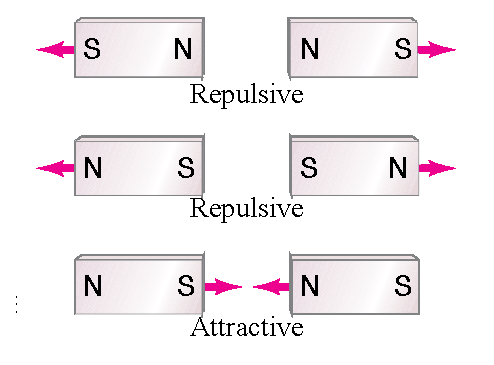
\includegraphics[width=0.6\linewidth]{2.eps}
  \captionof{figure}{Like poles of twomagnets repel; unlike poles attract.}
  \label{fig:20-2}
\end{minipage}
Physicists have searched for isolated single magnetic poles (monopoles), but no \textbf{magnetic monopole} has ever been observed. Besides iron, a few other materials, such as cobalt, nickel, gadolinium, andsome of their oxides and alloys, show strong magnetic effects. They are said to be \textbf{ferromagnetic} (from the Latin word ferrumfor iron). We can picture a \textbf{magnetic field} surrounding a magnet. Just as we drew electric field lines, we can also draw \textbf{magnetic field lines}, so that
\begin{enumerate}
  \item the direction of the magnetic field is tangent to a field line at any point, and 
  \item the number of lines per unit area is proportional to the strength of the magnetic field.
\end{enumerate}
\begin{minipage}{\linewidth}
  \vspace{0.5cm}
  \setlength{\abovecaptionskip}{0.2cm}
  \setlength{\belowcaptionskip}{0.3cm}
  \centering
  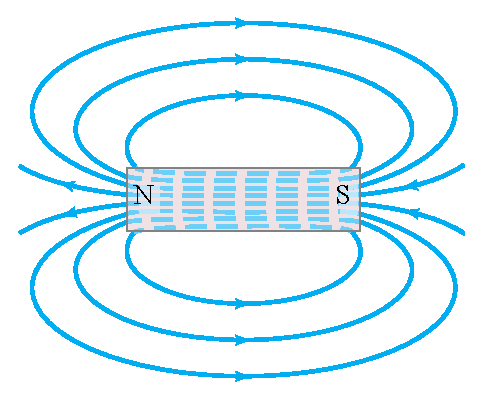
\includegraphics[width=0.6\linewidth]{4.eps}
  \captionof{figure}{Diagram ofmagnetic field lines for a bar magnet.}
  \label{fig:20-4}
\end{minipage}

\subsection{Earth’s Magnetic Field}
\begin{minipage}{\linewidth}
  \vspace{0.5cm}
  \setlength{\abovecaptionskip}{0.2cm}
  \setlength{\belowcaptionskip}{0.3cm}
  \centering
  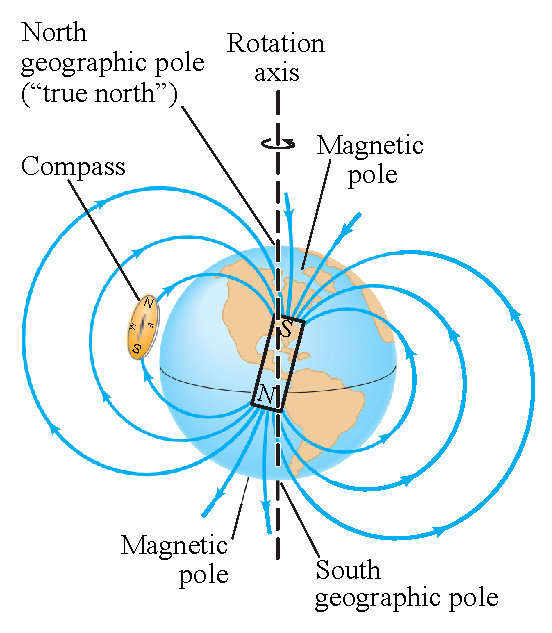
\includegraphics[width=0.6\linewidth]{5.eps}
  \captionof{figure}{The Earth acts like a huge magnet. But its magnetic poles are not at the geographic poles (on the Earth’s rotation axis).}
  \label{fig:20-5}
\end{minipage}
\subsection{Uniform Magnetic Field}
\begin{minipage}{\linewidth}
  \vspace{0.5cm}
  \setlength{\abovecaptionskip}{0.2cm}
  \setlength{\belowcaptionskip}{0.3cm}
  \centering
  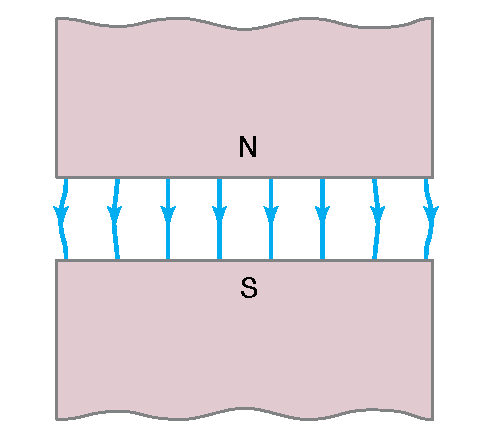
\includegraphics[width=0.6\linewidth]{7.eps}
  \captionof{figure}{Magnetic field between two wide poles of a magnet is nearly uniform, except near the edges.}
  \label{fig:20-7}
\end{minipage}
\section{Electric Currents Produce Magnetic Fields}
In 1820, Hans Christian Oersted (1777–1851) found that when a compass is placed near a wire, the compass needle deflects if (and only if) the wire carries an electric current, which showed that \textbf{an electric current produces a magnetic field}. There is a simple way to remember the direction of the magnetic field lines in this case. It is called a \textbf{right-hand rule} (See: Summary of RHRs - 1).
% \begin{minipage}{\linewidth}
%   \vspace{0.5cm}
%   \setlength{\abovecaptionskip}{0.2cm}
%   \setlength{\belowcaptionskip}{0.3cm}
%   \centering
%   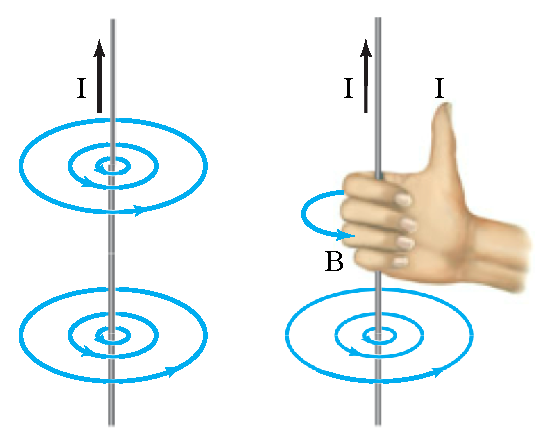
\includegraphics[width=0.6\linewidth]{8.eps}
%   \captionof{figure}{Right-hand rule for remembering the direction of the magnetic field: when the thumb points in the direction of the conventional current, the fingers wrapped around the wire point in the direction of the magnetic field. ($\vec { \mathbf { B } }$ is the symbol for magnetic field.}
%   \label{fig:20-8}
% \end{minipage}
\section{Force on an Electric Currentin a Magnetic Field; Definition of $\vec { \mathbf { B } }$}
A magnetic field exerts a force on an electric current. The SI unit for magnetic field is the \textbf{tesla} (T). For a straight wire of length l carrying a current I, the force has magnitude
\begin{equation}
  F = I \ell B \sin \theta,
\end{equation}
where $\theta$ is the angle between the magnetic field $\vec { \mathbf { B } }$ and the current direction. The direction of the force is perpendicular to the current-carrying wire and to the magnetic field, and is given by another right-hand rule (See: Summary of RHRs - 2). Equation (1) serves as the definition of B
magnetic field $\vec { \mathbf { B } }$.
\section{Force on an Electric Charge Moving in a Magnetic Field}
Similarly, a magnetic field exerts a force on a charge q moving with velocity v of magnitude
\begin{equation}
F = q v B \sin \theta,
\end{equation}
where $\theta$ is the angle between $\vec { \mathbf { v } }$ and $\vec { \mathbf { B } }$. The direction of $\vec { \mathbf { F } }$ is perpendicular to $\vec { \mathbf { v } }$ and to $\vec { \mathbf { B } }$  (again a right-hand rule; see: Summary of RHRs - 3). The path of a charged particle moving perpendicular to a uniform magnetic field is a circle.

\begin{minipage}{\linewidth}
  \vspace{0.5cm}
  \setlength{\abovecaptionskip}{0.2cm}
  \setlength{\belowcaptionskip}{0.3cm}
  \centering
  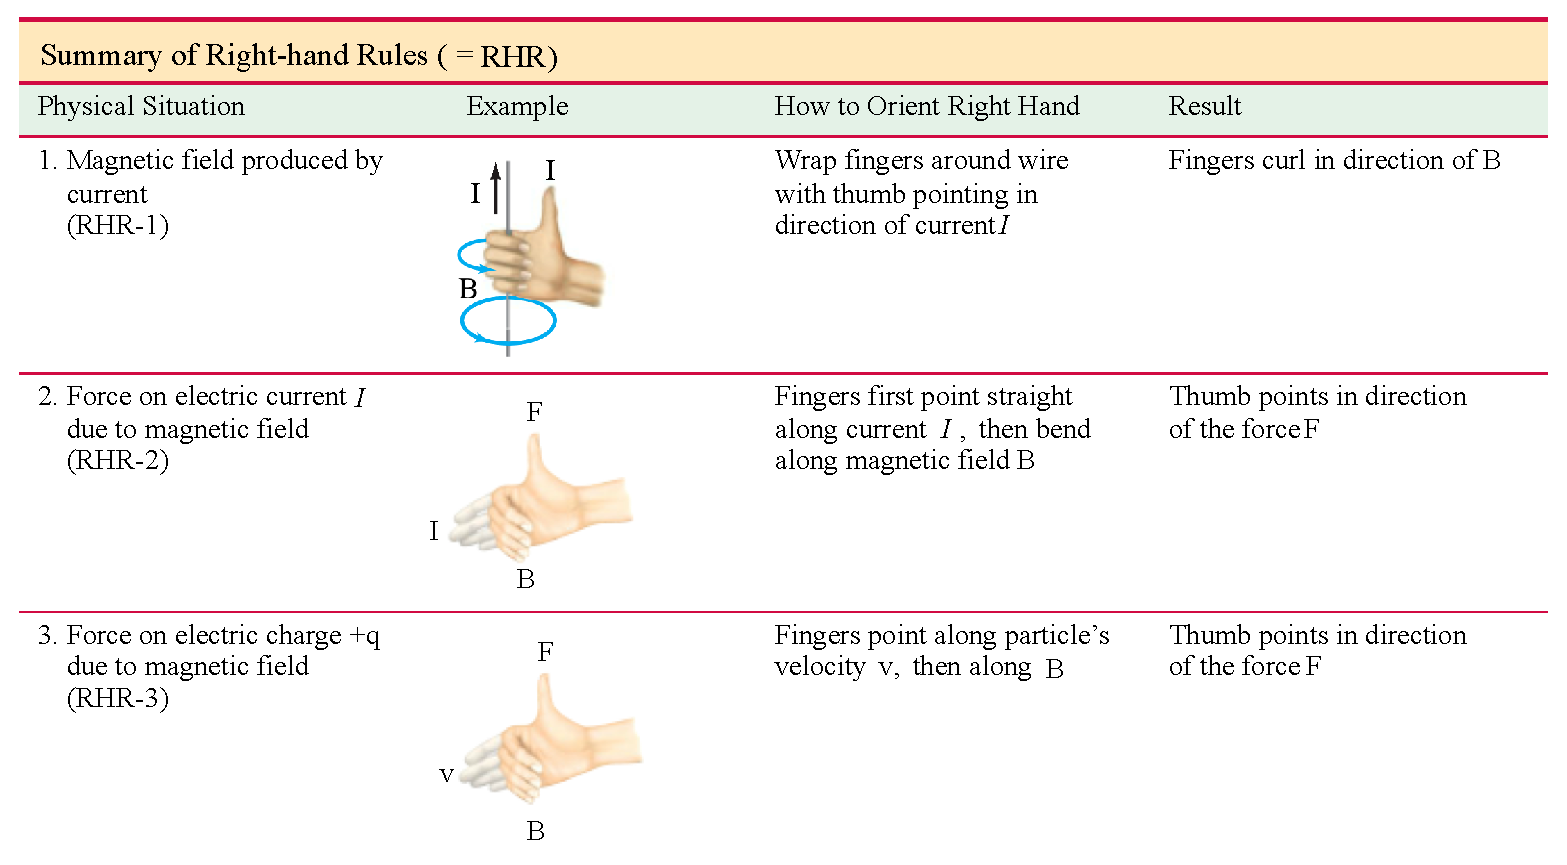
\includegraphics[width=\linewidth]{RHR.eps}
  \captionof{figure}{Summary of RHRs.}
  \label{fig:20-8}
\end{minipage}

\section{Magnetic Field Due to a Long Straight Wire}
The magnitude of the magnetic field produced by a current $I$ in a long straight wire, at a distance $r$ from the wire, is
\begin{equation}
B = \frac { \mu _ { 0 } } { 2 \pi } \frac { I } { r }.
\end{equation}
The value of the constant $\mu _ { 0 }$, which is called the \textbf{permeability of free space}, is $\mu _ { 0 } = 4 \pi \times 10 ^ { - 7 } \mathrm { T } \cdot \mathrm { m } / \mathrm { A }$.
\section{Force between Two Parallel Wires}
The force $F_2$ exerted by $B_1$ on a length $l_2$ of wire 2, carrying current $I_2$ is
\begin{equation}
F _ { 2 } = \frac { \mu _ { 0 } } { 2 \pi } \frac { I _ { 1 } I _ { 2 } } { d } \ell _ { 2 }
\end{equation}
\begin{minipage}{\linewidth}
  \vspace{0.5cm}
  \setlength{\abovecaptionskip}{0.2cm}
  \setlength{\belowcaptionskip}{0.3cm}
  \centering
  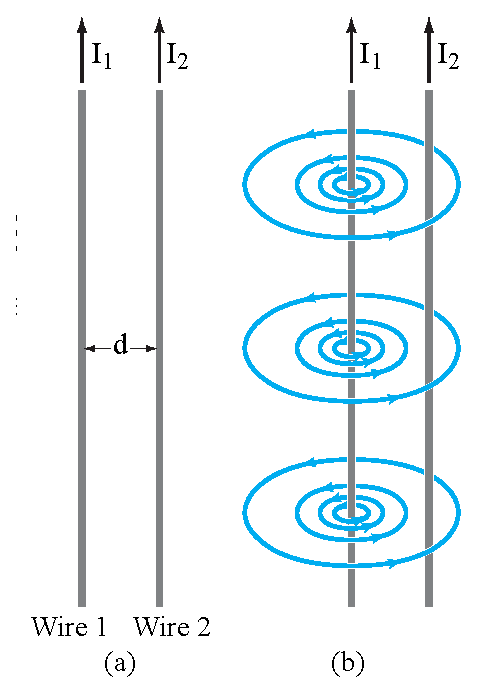
\includegraphics[width=0.6\linewidth]{26.eps}
  \captionof{figure}{(a) Two parallel conductors carrying currents $I_1$ and $I_2$. (b) Magnetic field $\vec { \mathrm { B } } _ { 1 }$ produced by $I_1$. (Field produced by I2 is not shown.) $\vec { \mathrm { B } } _ { 1 }$ points into page at position of $I_2$.}
  \label{fig:20-7}
\end{minipage}
\begin{minipage}{\linewidth}
  \vspace{0.5cm}
  \setlength{\abovecaptionskip}{0.2cm}
  \setlength{\belowcaptionskip}{0.3cm}
  \centering
  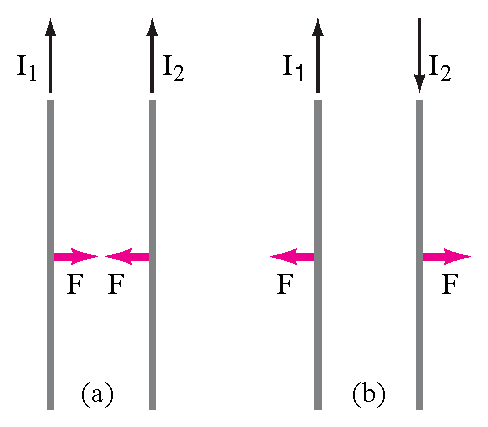
\includegraphics[width=0.6\linewidth]{27.eps}
  \captionof{figure}{(a) Parallel currents in the same direction exert an attractive force on each other. (b) Antiparallel currents (in opposite directions) exert a repulsive force on each other.}
  \label{fig:20-7}
\end{minipage}
\subsection{Definition of the Ampere and the Coulomb}
We use the force between two parallel current-carrying wires, Eq. (4), to define the ampere precisely. If $I _ { 1 } = I _ { 2 } = 1 \mathrm { A }$ exactly, and the two wires are exactly 1m apart, then
$$
\frac { F } { \ell } = \frac { \mu _ { 0 } } { 2 \pi } \frac { I _ { 1 } I _ { 2 } } { d } = \frac { \left( 4 \pi \times 10 ^ { - 7 } \mathrm { T } \cdot \mathrm { m } / \mathrm { A } \right) } { ( 2 \pi ) } \frac { ( 1 \mathrm { A } ) ( 1 \mathrm { A } ) } { ( 1 \mathrm { m } ) } = 2 \times 10 ^ { - 7 } \mathrm { N } / \mathrm { m }.
$$
Thus, \textit{one} \textbf{ampere} \textit{is defined as that current flowing in each of two long parallel wires, 1m apart, which results in a force of exactly $2 \times 10 ^ { - 7 } N$ per meter of length of each wire.} This is the precise definition of the ampere, and because it is readily reproducible, is called an \textbf{operational definition}. The \textbf{coulomb} is defined in terms of
the ampere as being exactly one ampere-second: $1 \mathrm { C } = 1 \mathrm { A } \cdot \mathrm { s }$.

\section{Solenoids and Electromagnets}
\section{Ampère’s Law}
\section{Torque on a Current Loop; Magnetic Moment}
\section{Applications: Motors, Loudspeakers, Galvanometers}

\end{multicols}

\end{document}